\section{Admin-Page}
\label{adminpage}


Ist der Benutzer als Admin angemeldet erscheint unter dem Vorschlag-Erstellen-Knopf ein 
\textit{Vorschlagsverwaltung/Park hinzufügen}-Knopf, welcher einen auf die \textit{Recommendation-View}
weiterleitet. 


\subsection{Recommendation-View}

\begin{figure}[H]
    \begin{center}
      \frame{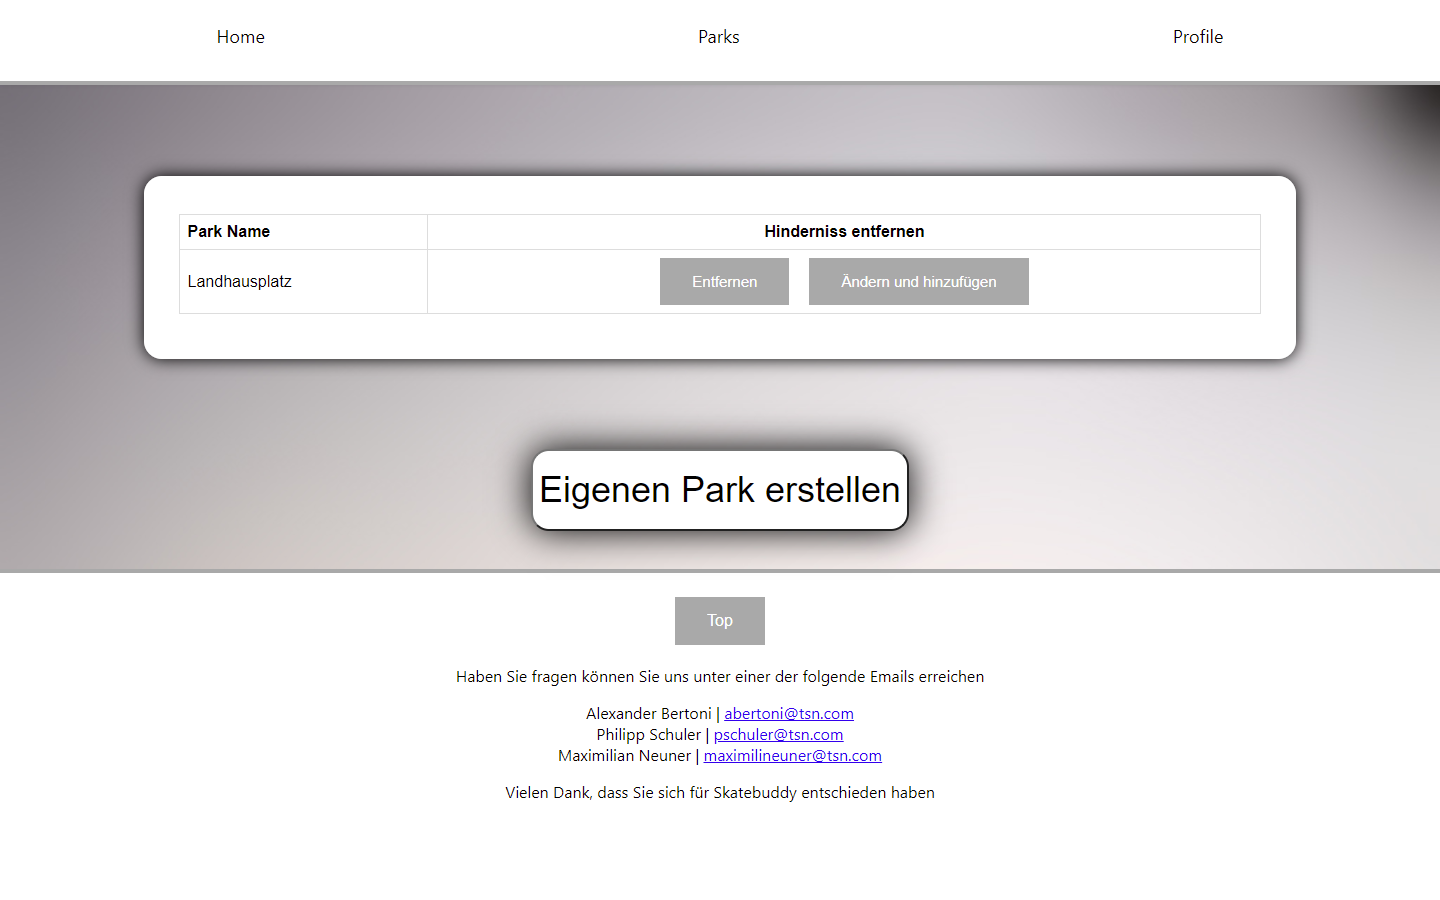
\includegraphics[width=1\textwidth]{Website/Recoom.png}}
      \caption{Liste der Vorschläge}
    \end{center}
\end{figure}

In dieser Ansicht kann der Admin alle erstellten Vorschläge der User einsehen. Er kann sie von hier 
aus löschen oder als Park hinzufügen. Er kann von hier aus auch selbst einen komplett neuen
Park hinzufügen, ohne einen Vorschlag zu bearbeiten.

\subsection{Park hinzufügen}

\begin{figure}[H]
    \begin{center}
      \frame{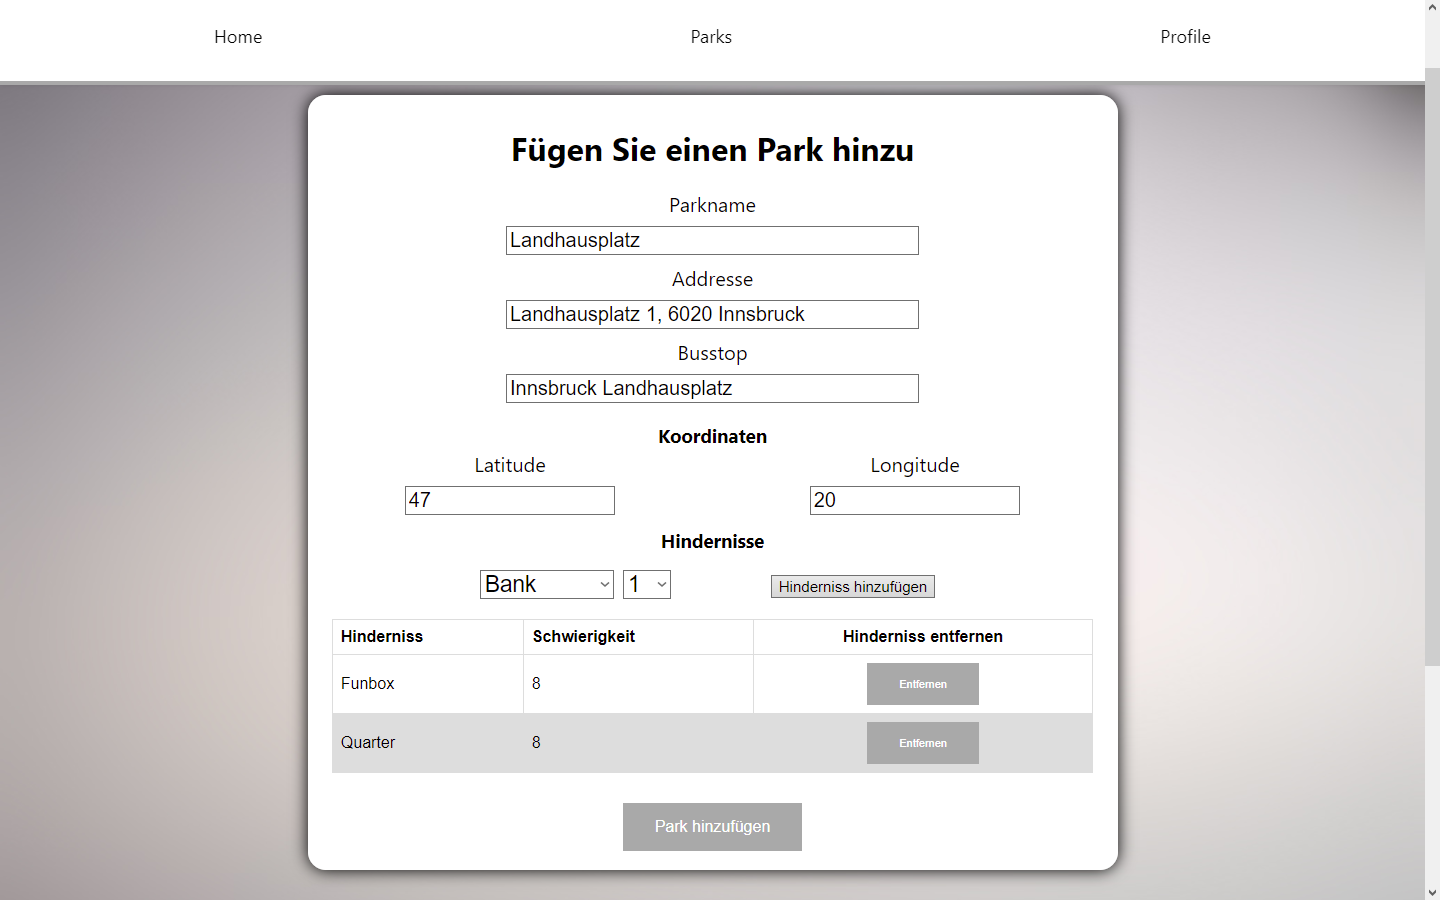
\includegraphics[width=1\textwidth]{Website/Recoom2.png}}
      \caption{Park erstellen}
    \end{center}
\end{figure}

Das Formular zum Park erstellen ist das Selbe wie dies zum Vorschläge erstellen. Benutzt der Admin einen 
Vorschlag welchen er bearbeiten möchte, werden die Daten des Vorschlages in die einzelnen Felder 
geladen und können somit bearbeitet werden. Wurde der Vorschlag fertig bearbeitet und als Park der 
Datenbank hinzugefügt, wird der bearbeitete Vorschlag aus der Datenbank gelöscht. 
Wird kein Vorschlag benutzt sondern ein komplett neuer Park erstellt, sind die Input Felder von Anfang 
an leer.
